\section{Synchronous Counters}
\label{sec:synchronous-counters}

\textit{Synchronous counters} are different from ripple counters in that clock pulses are applied to the inputs of all flip-flops.

\subsection{Binary Counter}
\label{subsec:binary-counter}

In a synchronous binary counter, the flip-flop in the least significant position is complemented with every pulse. A \textit{flip-flop in any other position is complemented when all the bits in the lower significant positions are equal to 1}. 

\begin{figure}[H]
  \centering
  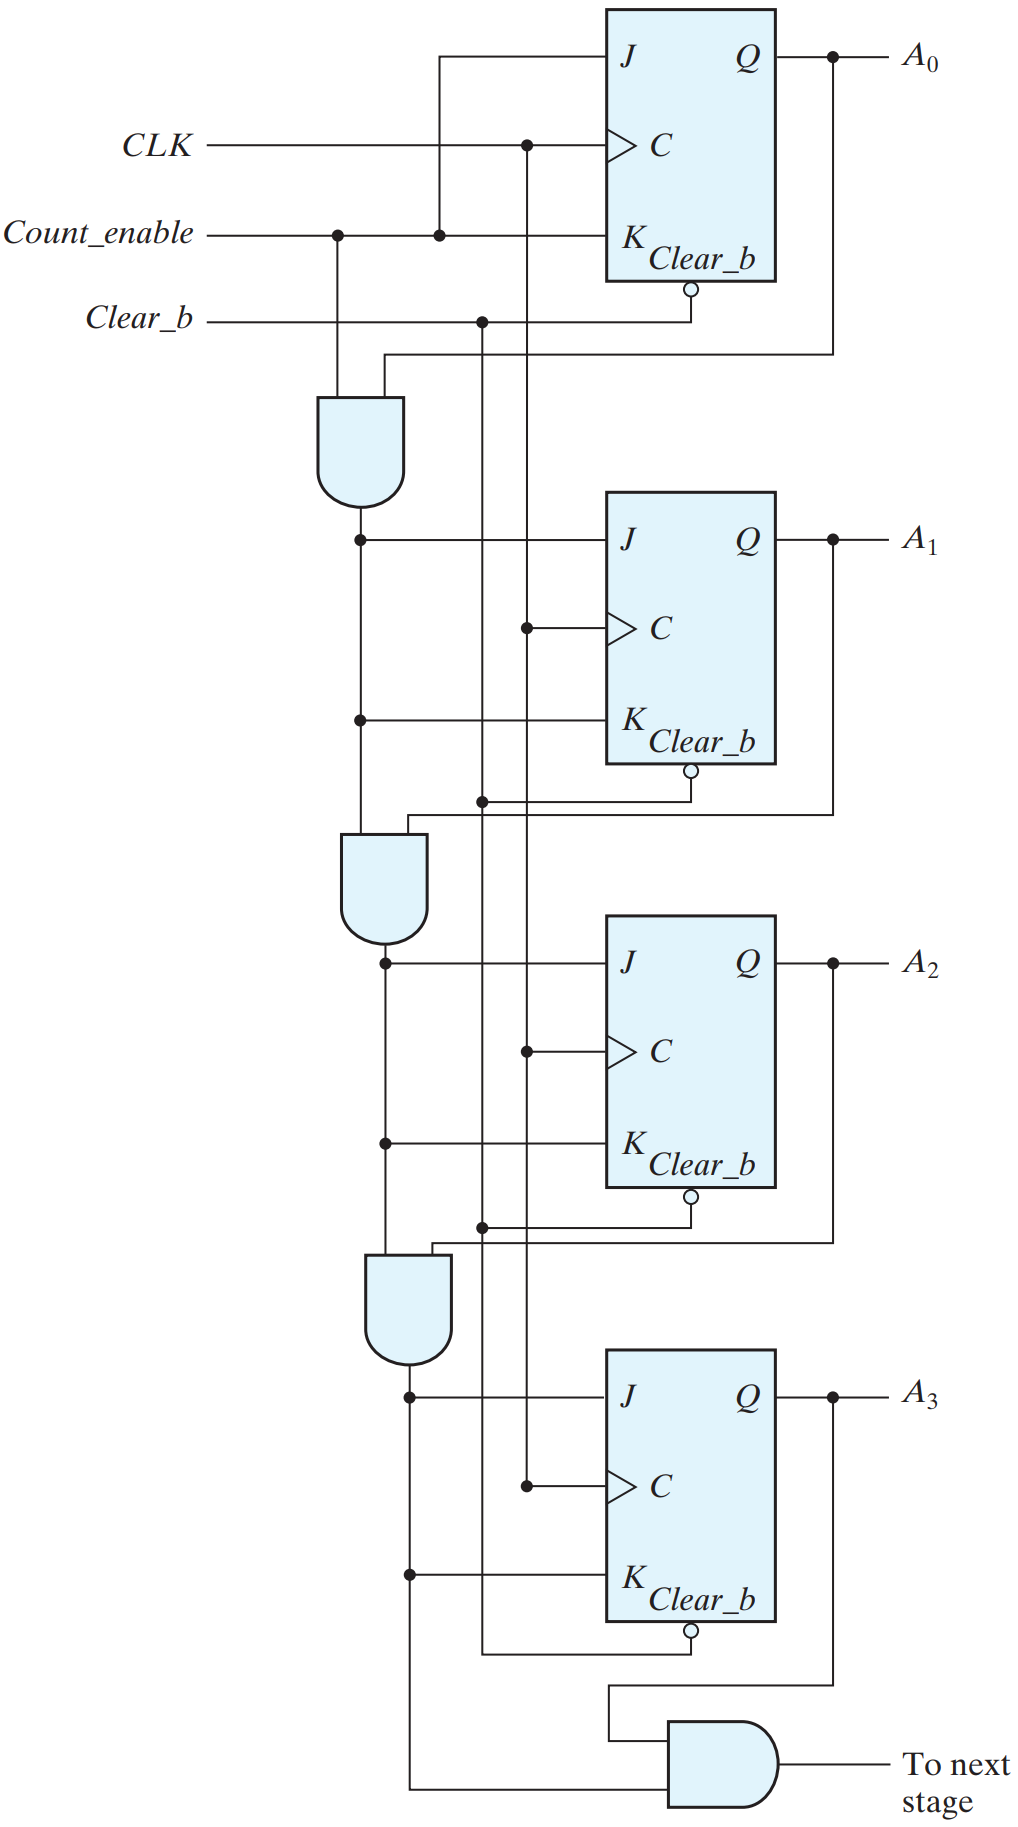
\includegraphics[width=.7\linewidth]{img/fig-6.12.png}
  \caption{Four-bit synchronous binary counter}
  \label{fig:6.12}
\end{figure}

\subsection{Up–Down Binary Counter}
\label{subsec:up-down-binary-counter}

A synchronous countdown binary counter goes through the binary states in reverse order, from 1111 down to 0000 and back to 1111 to repeat the count.

The bit in the least significant position is complemented with each pulse. \textit{A bit in any other position is complemented if all lower significant bits are equal to 0}.

A countdown binary counter can be constructed as shown in Fig. 12, except that the inputs to the AND gates must come from the complemented outputs, instead of the normal outputs, of the previous flip-flops. The two operations can be combined in one circuit to form a counter capable of counting either up or down. The circuit of an up–down binary counter using T flip-flops is shown in Fig. 13.

\begin{figure}[H]
  \centering
  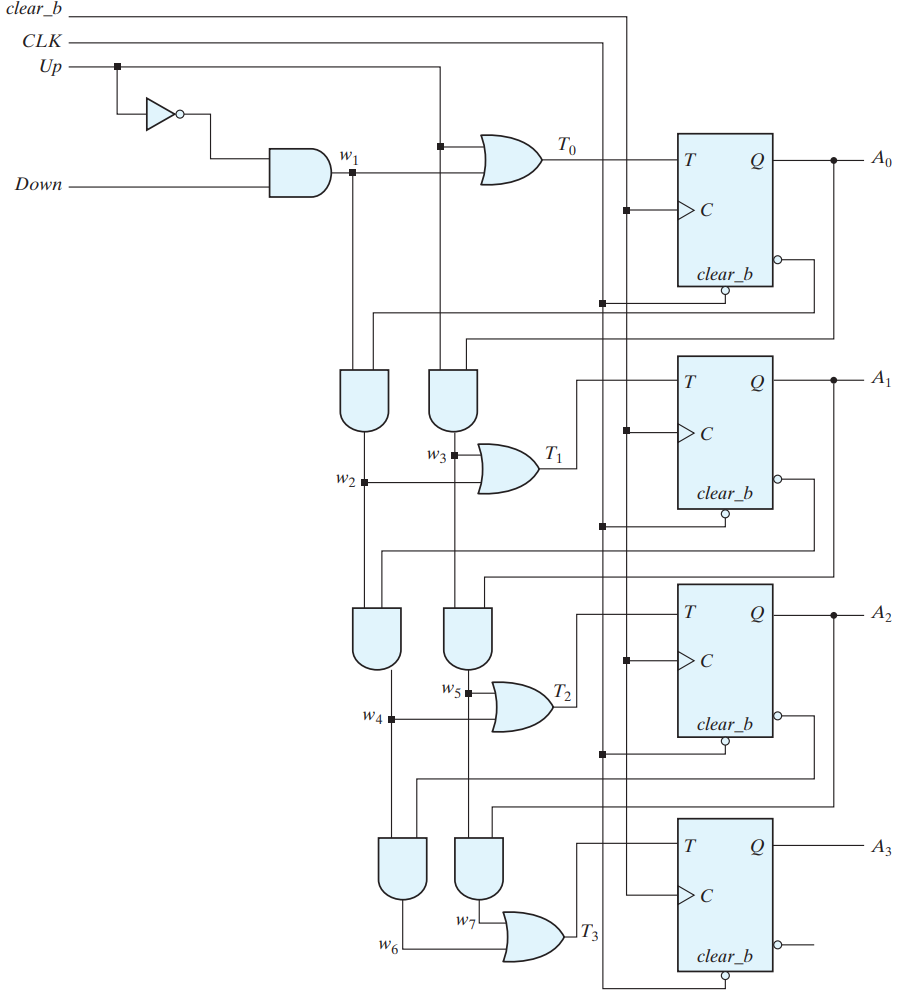
\includegraphics[width=\linewidth]{img/fig-6.13.png}
  \caption{Four-bit up–down binary counter}
  \label{fig:6.13}
\end{figure}

\subsection{BCD Counter}
\label{subsec:bcd-counter}

A BCD counter counts in binary-coded decimal from 0000 to 1001 and back to 0000. The state table of a BCD counter is listed in Table 6.5.

\begin{figure}[H]
  \centering
  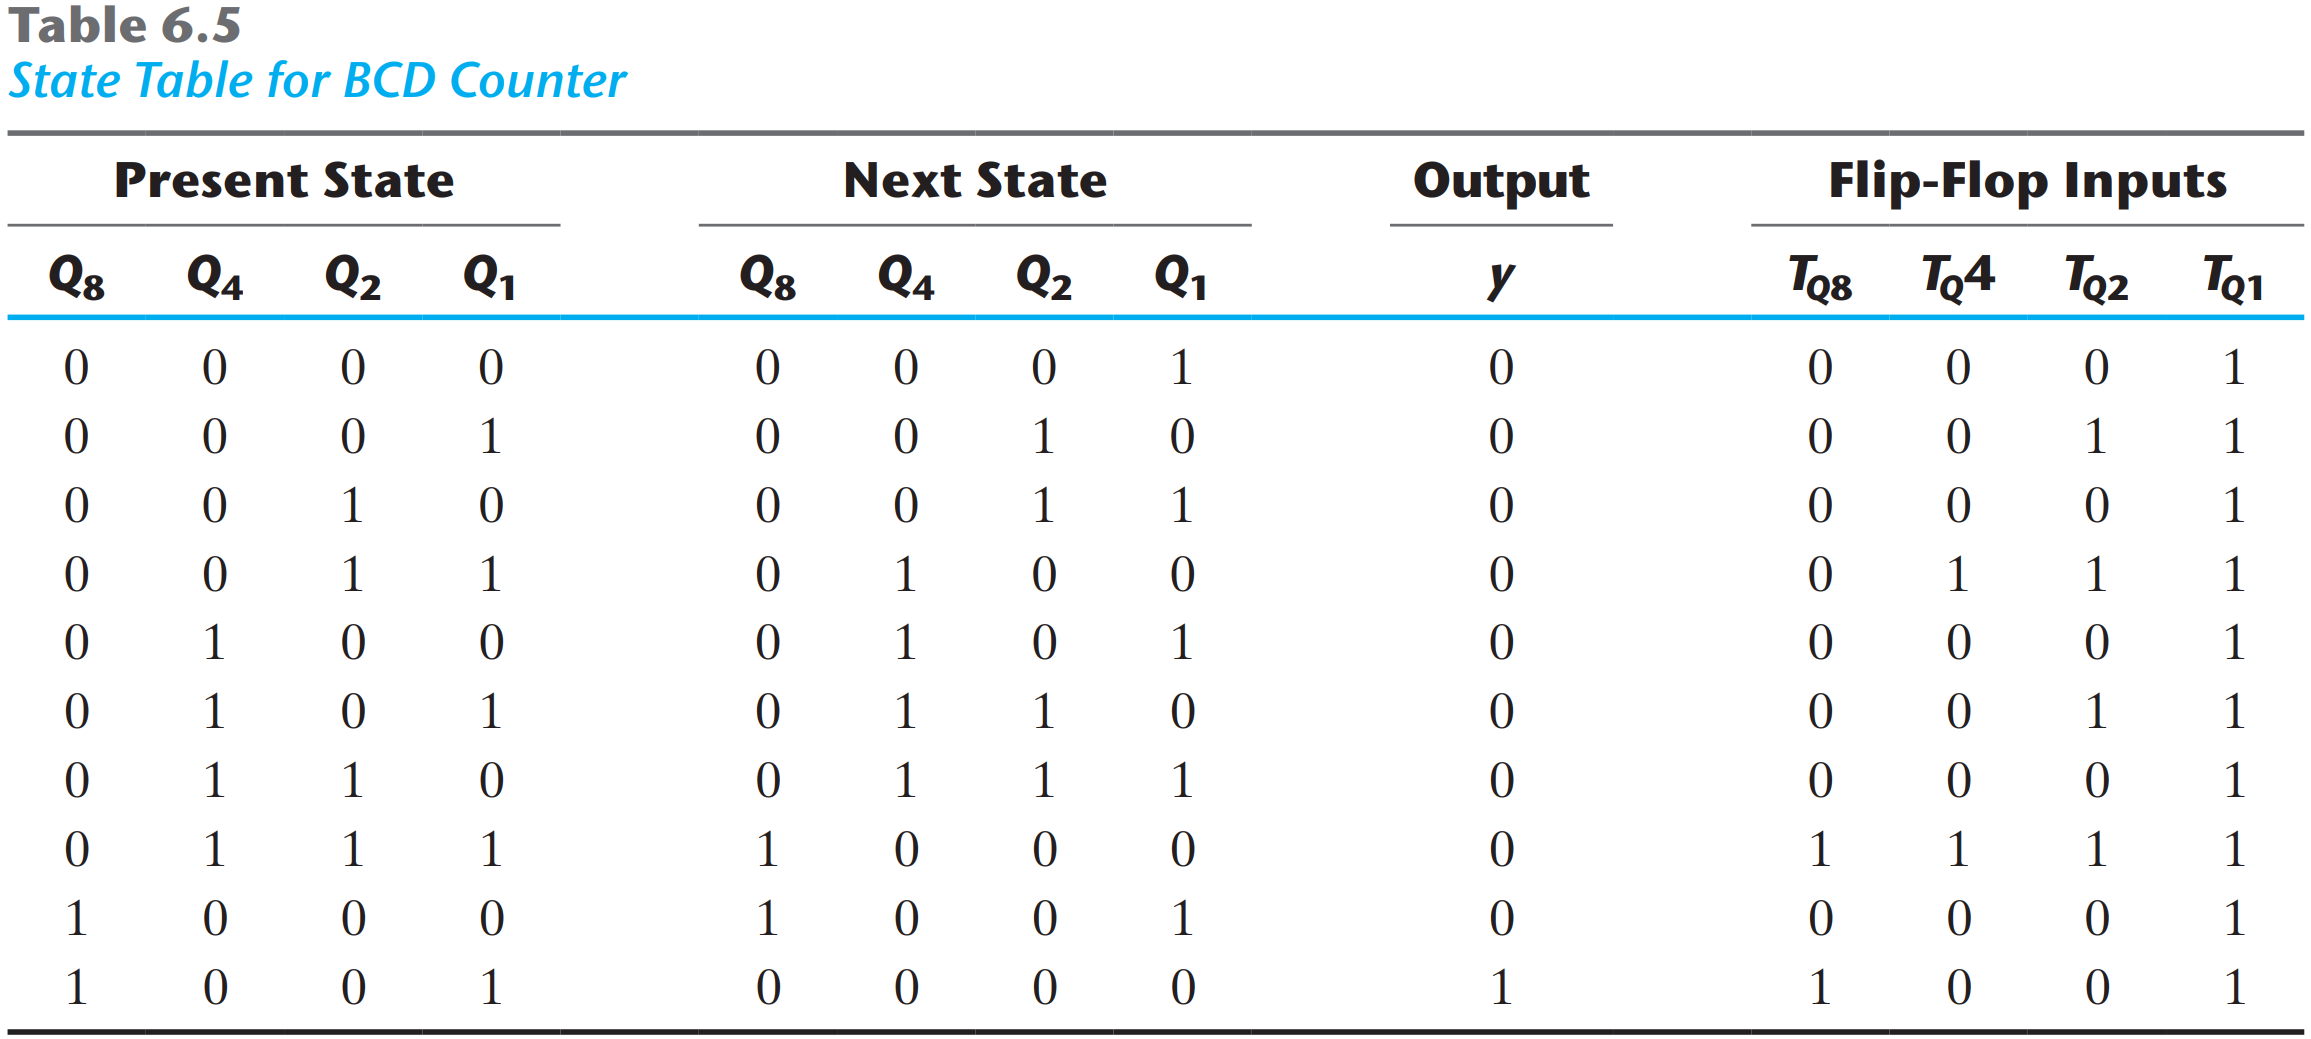
\includegraphics[width=.85\linewidth]{img/table-6.5.png}
  \label{table:6.5}
\end{figure}

The flip-flop input equations can be simplified:
\begin{align*}
  T_{Q_1} &= 1\\
  T_{Q_2} &= Q_8'Q_1\\
  T_{Q_4} &= Q_2Q_1\\
  T_{Q_8} &= Q_8Q_1 + Q_4Q_2Q_1\\
  y &= Q_8Q_1
\end{align*}
The circuit can easily be drawn with four $T$ flip-flops, five AND gates, and one OR gate.

\subsection{Binary Counter with Parallel Load}
\label{subsec:bin-counter-with-parallel-load}

Figure 14 shows the top-level block diagram symbol and the logic diagram of a four-bit register that has a parallel load capability and can operate as a binary counter.

\begin{figure}[H]
  \centering
  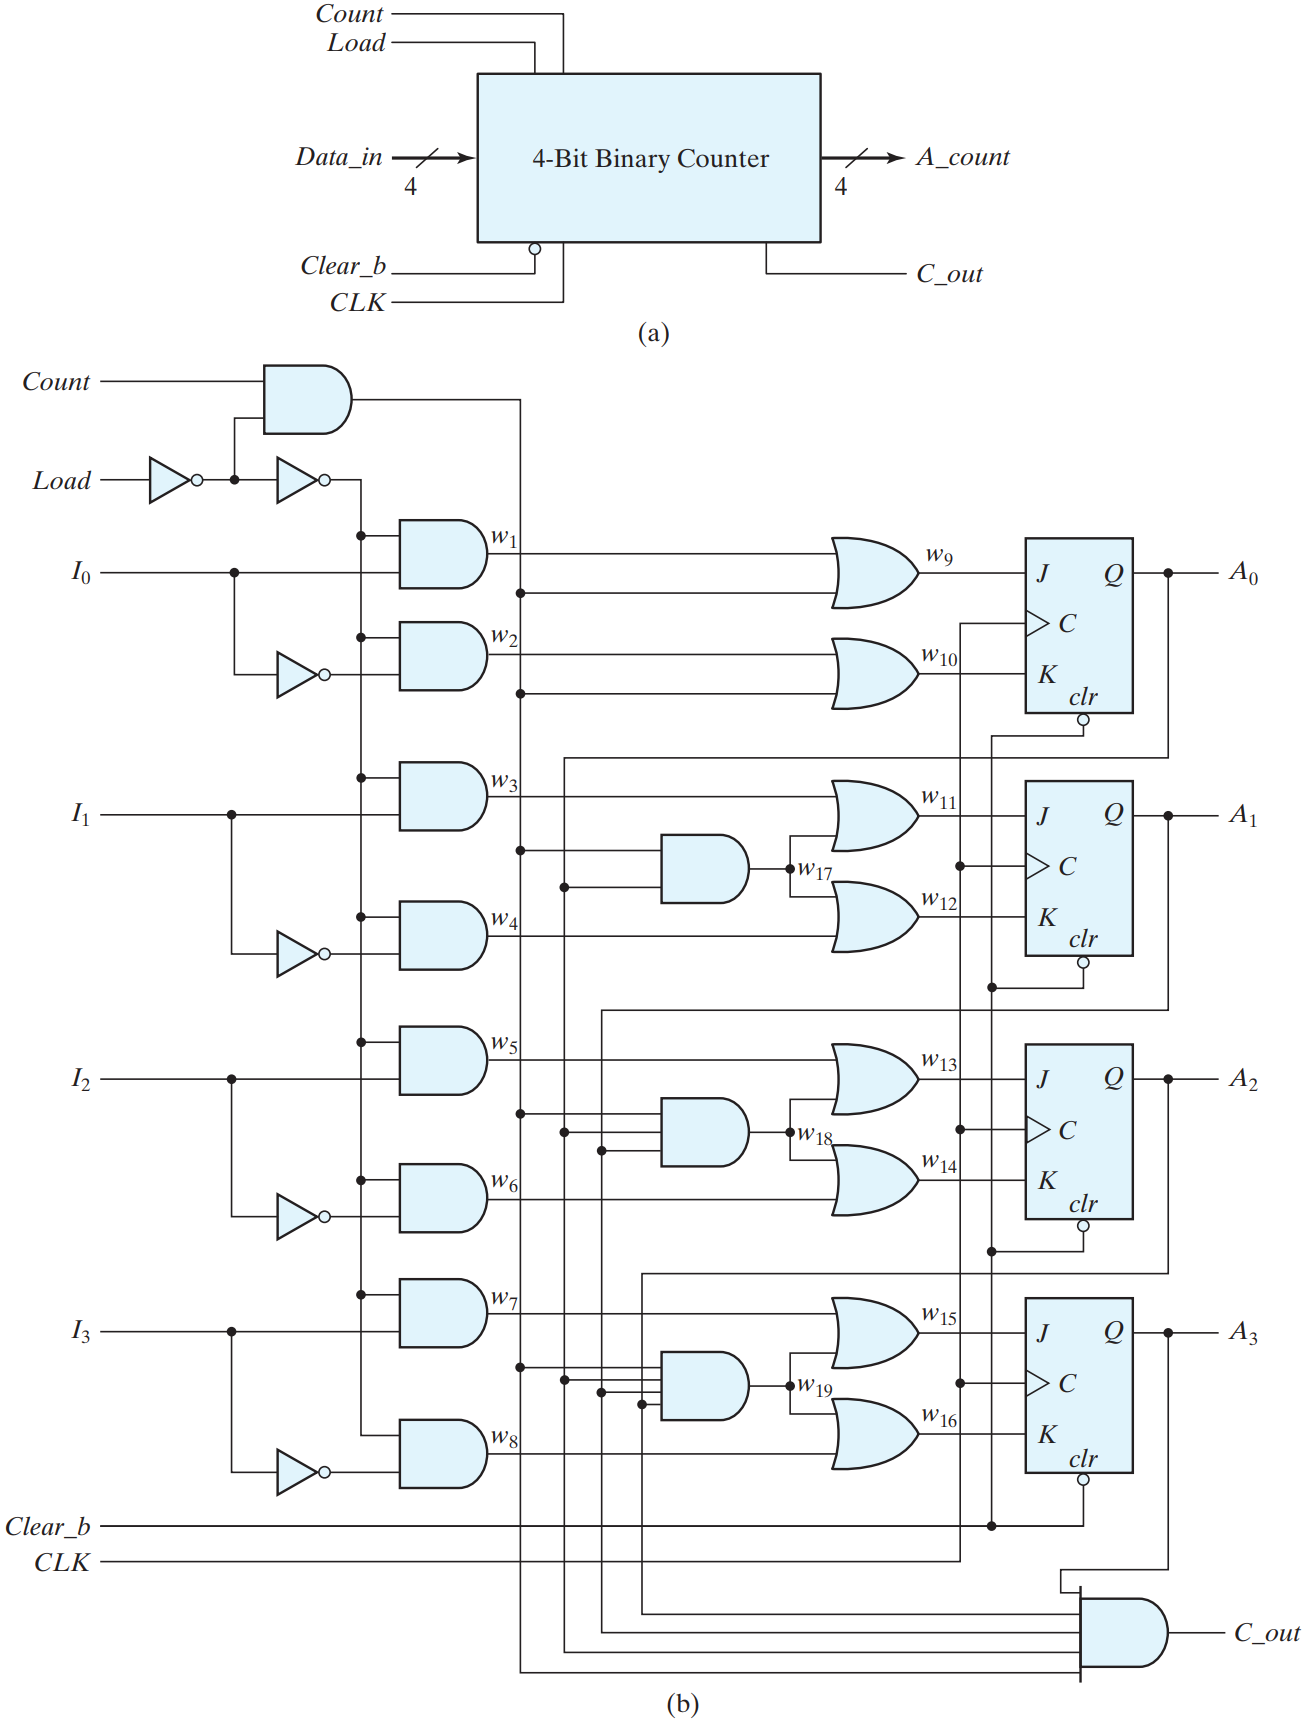
\includegraphics[width=\linewidth]{img/fig-6.14.png}
  \caption{Four-bit binary counter with parallel load}
  \label{fig:6.14}
\end{figure}

\noindent The operation of the counter is summarized in Table 6.6.

\begin{figure}[H]
  \centering
  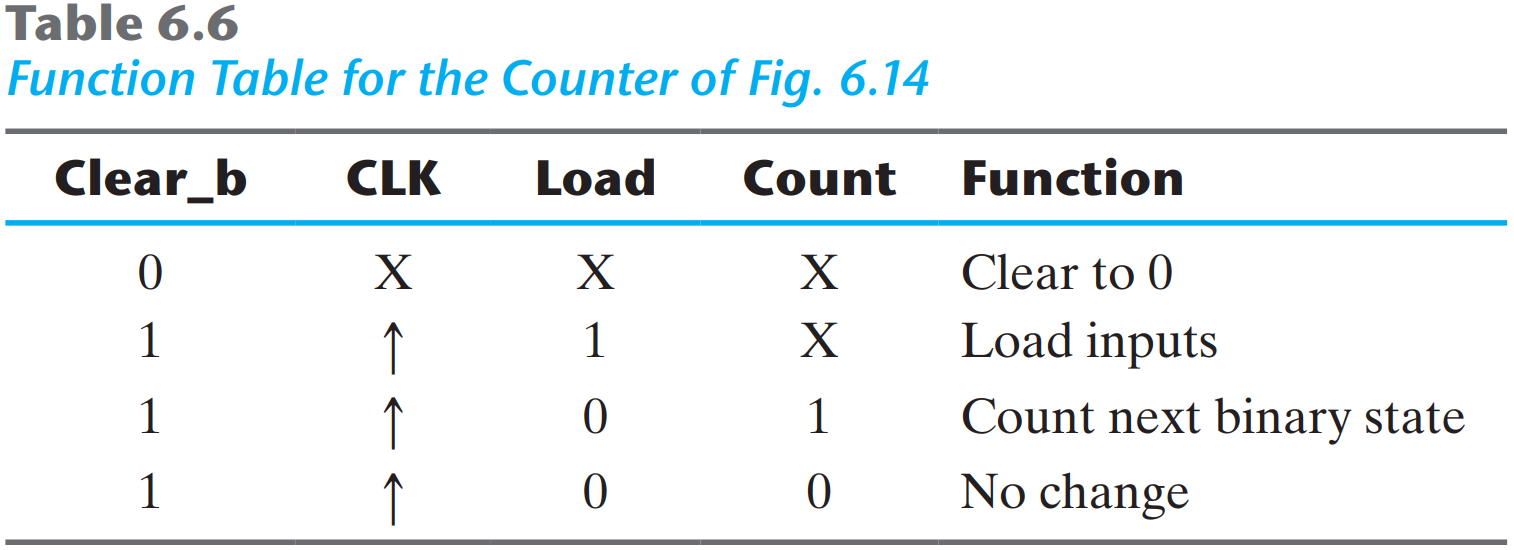
\includegraphics[width=\linewidth]{img/table-6.6.png}
  \label{table:6.6}
\end{figure}

\newpage

Figure 15 shows two ways in which a counter with a parallel load is used to generate the BCD count.
\begin{figure}[H]
  \centering
  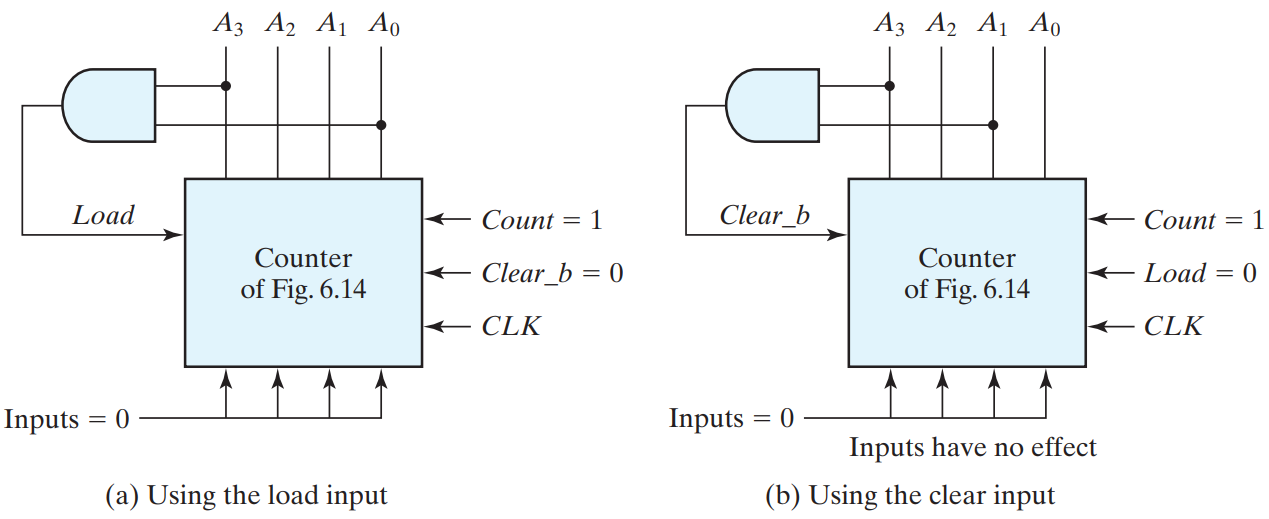
\includegraphics[width=\linewidth]{img/fig-6.15.png}
  \caption{Two ways to achieve a BCD counter using a counter with parallel load}
  \label{fig:6.15}
\end{figure}

